\documentclass[11pt]{article}
\usepackage{icmlko}
\begin{document}

\title{이미 최선이었다 --- 다른 목적으로 고른 표지가 전이를 제일 많이 산다}
\author{월드모델 실험실}
\date{노트 425 · 2026년 8월 3일}
\maketitle

\begin{abstract}
노트 424가 전이의 $0.39$ 를 \textbf{두 자리}(모바일 · 펀딩)로 좁혔다.
지금까지 잰 것은 \emph{나쁘게 바꾸는} 쪽뿐이었으니 위쪽을 쟀다 --- 그 자리에
다른 field 를 넣어 기준 $+0.1946$ 을 넘는지.

\begin{center}
\begin{tabular}{llr}
\hline
자리 & 후보 & KR 전이 \\
\hline
\textbf{모바일} & \textbf{무료 여부 (현행)} & $\mathbf{+0.1946}$ \\
 & \texttt{n\_genre} & $+0.1116$ \\
 & \texttt{advisory} & $+0.0764$ \\
\hline
\textbf{펀딩} & \textbf{\texttt{category} (현행)} & $\mathbf{+0.1946}$ \\
 & \texttt{n\_delivery} & $+0.0927$ \\
 & \texttt{n\_reward} & $+0.0922$ \\
 & \texttt{adult\_only} & $+0.0817$ \\
\hline
\end{tabular}
\end{center}

\textbf{다섯 후보가 두 자리에서 모두 진다.} 사전 등록의 실패 조건 그대로다
--- \emph{셋 다 못 넘으면 현행 선택이 이미 쓸 수 있는 것 중 최선이고,
전이를 더 사려면 다른 종류의 자료를 모아야 한다.}
\end{abstract}

\section{누가 고른 것인가}

여기서 걸리는 것이 있다. \textbf{현행 field 는 전이를 보고 고른 것이
아니다.} 노트 138이 ``집단만 아는 예측기''라는 \emph{바닥선}을 만들려고
손으로 골랐고, 기준은 하나였다 --- \emph{라벨 눈금이 기계적으로 갈리는
자리, 전부 기획 시점에 아는 것.} 전이라는 말은 그 노트에 없다.

그런데 그 선택이 내가 찾아낸 모든 대안을 이긴다. 둘 중 하나다: 운이 좋았거나,
\textbf{``기획 시점에 라벨을 가르는 자리''라는 기준이 마침 전이의 기준이기도
하거나.} 지금 자료로는 못 가른다 --- 후보가 자리마다 서넛뿐이다.

\section{판은 이 축에서 거의 눈이 멀었다}

판과 전이를 둘 다 잰 표지 구성 다섯을 모으면 폭이 이렇다.

\begin{center}
\begin{tabular}{lr}
\hline
판의 폭 & $0.0028$ \\
전이의 폭 & $0.3888$ \\
\hline
\textbf{비} & $\mathbf{139}$ 배 \\
\hline
\end{tabular}
\end{center}

판의 폭 전체가 씨앗 잡음($\pm 0.0007$)의 \textbf{두 배}다. 그 안에서
전이는 $+0.20$ 에서 $-0.19$ 까지 간다. 노트 423이 두 점으로 말한 것이
다섯 점에서 그대로다 --- \textbf{순위 지표로는 이 선택을 할 수 없다.}

\section{그래서 다음은 자료다}

field 를 바꿔 전이를 더 사는 길은 \textbf{닫혔다.} 지금 레코드에 든 기획
시점 범주 중 쓸 만한 것은 이미 쓰고 있다. 남은 길 둘:

\begin{tabular}{lp{7.0cm}}
\hline
새 자료 & 지금 레코드에 없는 기획 시점 범주를 모은다. 어떤 종류가 전이를
사는지는 아직 모르니 \textbf{모으기 전에 기준이 필요하다} \\
표지 아닌 길 & 전이를 사는 것이 표지뿐인지 안 재 봤다. 노트 417~425는
전부 표지 이야기다 \\
세 번째 전이 짝 & 여전히 없다. 두 짝(KR 만화 · 비게임 앱)으로 $0.39$ 짜리
결론을 지고 있다 \\
\hline
\end{tabular}

\begin{figure}[h]
\centering
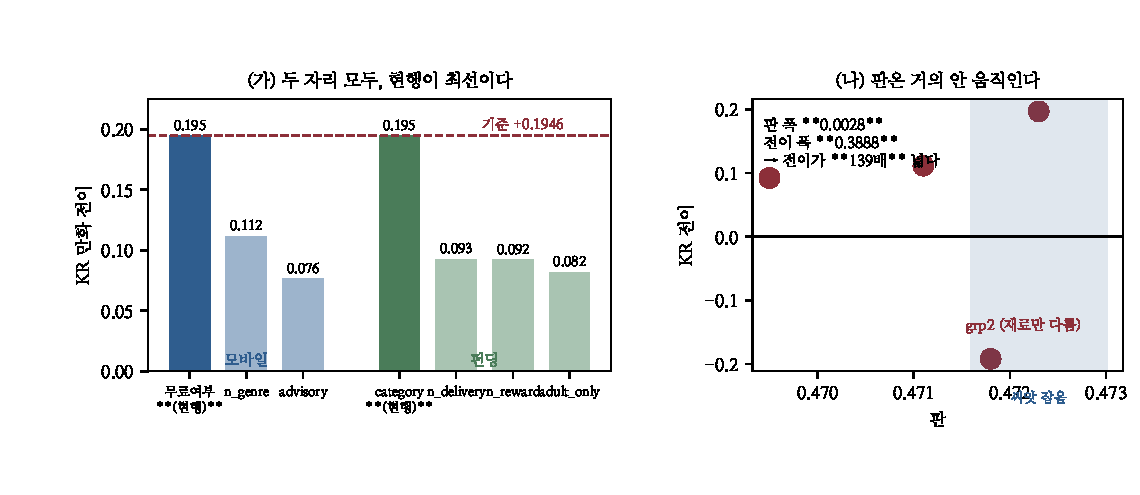
\includegraphics[width=\textwidth]{figs/fig425.pdf}
\caption{(가) 두 자리 모두 현행이 최선. (나) 다섯 구성의 판과 전이 ---
판은 씨앗 잡음의 두 배 안에 모여 있는데 전이는 부호가 뒤집힌다.}
\end{figure}

\end{document}
